%câu 33
\begin{ex}%[2D4N3-1]
	Cho hình phẳng được tô màu trong hình bên dưới
	\begin{center}
		\begin{tikzpicture}[font=\footnotesize, line join=round, line cap=round, >=stealth, scale = 0.8]
		\draw[->] (-1.5,0) --(0,0) node[below right]{$O$}--(1.5,0) node[below]{$x$};
		\draw[->] (0,-.7) --(0,3.2) node[right]{$y$};
		\draw[fill = black] (1,0) node[below]{$1$} circle (1pt);
		\draw[fill = black] (-1,0) node[below left]{$-1$} circle (1pt);
		\draw[fill = black] (0,1) node[left]{$1$} circle (1pt);
		\draw[fill = black] (0,0) circle (1pt);
		\draw[dashed](1,0)--(1,2.71) (-1,0)--(-1,0.37);
		%	\clip (-1.3,-.4) rectangle (1.5,4);
		\draw [samples=100, domain=-1.2:1.1] plot (\x, {e^(\x)});
		\fill[pattern = north west lines] (-1,0) -- plot[smooth,samples=100,domain=-1:1] (\x, {e^(\x)}) -- (1,0) -- cycle;
		\draw (1.3,3)node[above]{\scriptsize $ y=e^x $};
	\end{tikzpicture}
	\end{center}
Các mệnh đề sau đây đúng hay sai?
\choiceTF
{Hình phẳng được tô màu trong hình vẽ trên được giới hạn bởi các đồ thị $ y=\mathrm{e}^x $; $ y=0 $; $ x=0 $; $ x=1 $}
{\True Diện tích hình phẳng tô màu trong hình vẽ là $ \displaystyle\int\limits_{-1}^1 \mathrm{e}^x \mathrm{\,d}x$}
{Diện tích hình phẳng tô màu trong hình vẽ là $ \displaystyle\int\limits_0^1 \mathrm{e}^x \mathrm{\,d}x$}
{\True Hình phẳng được tô màu trong hình vẽ trên được giới hạn bởi các đồ thị $ y=\mathrm{e}^x $; $ y=0 $; $ x=-1 $; $ x=1 $}
\loigiai{
\begin{itemchoice}
\itemch Sai. Vì hình phẳng được tô màu trong hình vẽ trên được giới hạn bởi các đồ thị $ y=\mathrm{e}^x $; $ y=0 $; $ x=-1 $; $ x=1 $.
\itemch Đúng. Ta có $ S=\displaystyle\int\limits_{-1}^1 \mathrm{e}^x \mathrm{d}x $.
\itemch Sai.
\itemch Đúng.
\end{itemchoice}}
\end{ex}

%CÂU 34
\begin{ex}%[2D4N3-1]
	Cho hình phẳng được tô màu trong hình bên dưới.
	\begin{center}
		\begin{tikzpicture}[font=\footnotesize, line join=round, line cap=round, >=stealth, scale = 0.8]
			\draw[->] (-.5,0) --(0,0) node[below right]{$O$}--(3.3,0) node[below]{$x$};
			\draw[->] (0,-.7) --(0,4) node[right]{$y$};
			\draw[fill = black] (2,0) node[below left]{$2$} circle (1pt);
			\draw[fill = black] (0,1) node[left]{$1$} circle (1pt);
			\draw[fill = black] (0,0) circle (1pt);
			\draw[dashed](2,0)--(2,3);
			\fill[pattern=north west lines] plot[domain=2:0](\x,{0.5^(\x)})-- plot[domain=0:2](\x,{(\x)+1}) --cycle;
			\draw [samples=100, domain=-.2:2.6] plot (\x, {(\x)+1});
			\draw [samples=100, domain=-.2:2.8] plot (\x, {0.5^(\x)});
			\draw (1.5,2.6)node[above,rotate=45]{\scriptsize $ y=x+1 $};
			\draw (3.3,.02)node[above]{\scriptsize $ y=\left(\dfrac{1}{2}\right)^x $};
		\end{tikzpicture}
	\end{center}
Các mệnh đề sau đúng hay sai?
\choiceTF
{\True Hình phẳng được tô màu trong hình vẽ trên được giới hạn bởi các đồ thị $ y=x+1 $; $ y=\left(\dfrac{1}{2}\right)^x $; $ x=0 $; $ x=2 $}
{Diện tích hình phẳng tô màu trong hình vẽ là $ \displaystyle\int\limits_0^2\left[\left(\dfrac{1}{2}\right)^x-x-1\right]\mathrm{\,d}x$}
{\True Diện tích hình phẳng tô màu trong hình vẽ bằng $ S=4-\dfrac{3}{4\ln 2}$}
{Hình phẳng được tô màu trong hình vẽ trên được giới hạn bởi các đồ thị $ y=x+1 $; $ y=\left(\dfrac{1}{2}\right)^x $; $ x=1 $; $ x=2 $}
\loigiai{
\begin{itemchoice}
	\itemch Đúng. Vì hình phẳng được tô màu trong hình vẽ trên được giới hạn bởi các đồ thị $ y=x+1 $; $ y=\left(\dfrac{1}{2}\right)^x $; $ x=0 $; $ x=2 $.
	\itemch Sai. Trên đoạn $ \left[0;2\right] $, đồ thị hàm số $ y=x+1 $ nằm trên đồ thị hàm số $ y=\left(\dfrac{1}{2}\right)^x $ nên với mọi $ x \in \left[0;2\right]$ ta có $ x+1 \ge \left(\dfrac{1}{2}\right)^x  \Rightarrow \left|\left(\dfrac{1}{2}\right)^x-(x+1)\right|=x+1-\left(\dfrac{1}{2}\right)^x$.\\
	Vậy diện tích hình phẳng tô màu là $ \displaystyle\int\limits_0^2\left[ x+1-\left(\dfrac{1}{2}\right)^x\right]\mathrm{\,d}x$.
	\itemch Đúng. Ta có $ S=\displaystyle\int\limits_0^2\left[ x+1-\left(\dfrac{1}{2}\right)^x\right]\mathrm{\,d}x=\left( \dfrac{x^2}{2}+x+\dfrac{2^{-x}}{\ln 2}\right) \Bigg|_0^2 =4+\dfrac{1}{4\ln 2}-\dfrac{1}{\ln2}=4-\dfrac{3}{4\ln 2}$.
	\itemch Sai.
\end{itemchoice}
}
\end{ex}

%Câu 35
\begin{ex}%[2D4H3-1]
Cho đồ thị hàm số $y=f(t)$ như hình vẽ.
\begin{center}
	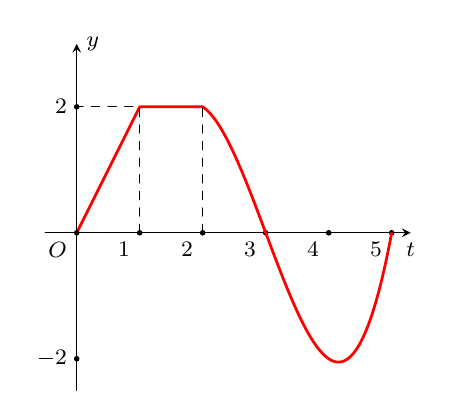
\begin{tikzpicture}[font=\footnotesize, line join=round, line cap=round, >=stealth, scale = 0.8]
		\draw[->] (-.5,0) --(0,0) node[below left]{$O$}--(5.3,0) node[below]{$t$};
		\draw[->] (0,-2.5) --(0,3) node[right]{$y$};
		\draw[fill = black] (1,0) node[below left]{$1$} circle (1pt) (2,0) node[below left]{$2$} circle (1pt) (3,0) node[below left]{$3$} circle (1pt) (4,0) node[below left]{$4$} circle (1pt) (5,0) node[below left]{$5$} circle (1pt);
		\draw[fill = black] (0,2) node[left]{$2$} circle (1pt) (0,-2) node[left] {$-2$} circle (1pt);
		\draw[line width = 1pt, red] (0,0)--(1,2)--(2,2);
		\draw[fill = black] (0,0) circle (1pt);
		\draw[line width = 1pt, red] 
		plot[domain=2:5, samples=100] (\x, {2/3*((\x)^3-9*(\x)^2+23*(\x)-15)});
		\draw[dashed] (1,0)--(1,2)--(0,2) (2,0)--(2,2);
	\end{tikzpicture}
\end{center}
Các mệnh đề sau đây đúng hay sai?
\choiceTF
{\True Diện tích hình phẳng được giới hạn các đồ thị hàm số $y=f(t)$, trục $O t$ và hai đường thẳng $t=0$; $t=1$ là $S=\dfrac{1}{2} \displaystyle\int\limits_{0}^{1} t \mathrm{\,d} t=\dfrac{1}{4}$}
{\True Diện tích hình phẳng được giới hạn các đồ thị hàm số $y=f(t)$, trục $Ot$ và hai đường thẳng $t=1$; $t=2$ là $S=\displaystyle\int\limits_{1}^{2} 2 \mathrm{\,d}t=2$}
{\True Tích phân $\displaystyle\int\limits_{2}^{3} f(x) \mathrm{\,d} x$ biểu thị cho phần diện tích của hình phẳng giới hạn các đồ thị hàm số $y=f(t)$, trục $O t$ và hai đường thẳng $t=2$; $ t=3$}
{Tích phân $\displaystyle\int\limits_{3}^{5} f(x) \mathrm{\,d} x$ biểu thị cho phần diện tích của hình phẳng giới hạn các đồ thị hàm số $y=f(t)$, trục $O t$ và hai đường thẳng $t=3$; $ t=5$}
\loigiai{
	\begin{itemchoice}
		\itemch Đúng. Vì đồ thị hàm số $y=f(t)$ trên đoạn $\left[0 ; 1\right]$ là $y=\dfrac{1}{2} t$. Do đó diện tích hình phẳng được giới hạn các đồ thị hàm số $y=f(t)$, trục $Ot$ và hai đường thẳng $t=0$; $t=1$ là $S=\dfrac{1}{2}\displaystyle\int\limits_{0}^{1} t \mathrm{\,d} t=\dfrac{1}{4}$.
		\itemch Đúng. Vì trên đoạn $ \left[1;2\right] $ đồ thị hàm số $y=f(t)=2$ nên hình phẳng được giới hạn bởi các đồ thị hàm số $ y=f(t) $, trục $O t$ và hai đường thẳng $t=1$; $t=2$ có diện tích là $S=\displaystyle\int\limits_{1}^{2} 2 \mathrm{\,d}t=2$.
		\itemch Đúng. Tích phân $\displaystyle\int\limits_{2}^{3} f(x) \mathrm{\,d} x=\displaystyle\int\limits_{2}^{3} f(t) \mathrm{\,d} t$ nên giá trị của tích phân $\displaystyle\int\limits_{2}^{3} f(t) \mathrm{\,d} t$ là diện tích của hình phẳng giới hạn các đồ thị hàm số $y=f(t)$, trục $Ot$ và hai đường thẳng $t=2$; $t=3$.
		\itemch Sai. Tích phân $\displaystyle\int\limits_{3}^{5} f(x) \mathrm{\,d} x=\displaystyle\int\limits_{3}^{5} f(t) \mathrm{\,d} t$.\\
		Diện tích hình phẳng được giới hạn các đồ thị hàm số $y=f(t)$, trục $O t$ và hai đường thẳng $t=3$; $t=5$ là $S=\displaystyle\int\limits_{3}^{5} \left|f(t)\right| \mathrm{\,d} t$.
	\end{itemchoice}
}
\end{ex}

\Closesolutionfile{ans}
\indapan{3}{ans/ans-2-C4B3CD1_10-19-DS}

\Opensolutionfile{ans}[ans/ans-C4B3CD1_20-26-KQ]
\TNSA
%Câu 36

\begin{ex}%[2D4N3-1]
Tính diện tích hình phẳng được tô màu trong hình bên dưới.
\begin{center}
	\begin{tikzpicture}[font=\footnotesize, line join=round, line cap=round, >=stealth, scale = 1]
		\draw[->] (-.5,0) --(0,0) node[below left]{$O$}--(2.7,0) node[below]{$x$};
		\draw[->] (0,-.5) --(0,2.5) node[right]{$y$};
		\draw[fill = black] (1,0) node[below]{$1$} circle (1pt) (2,0) node[below]{$2$} circle (1pt);
		\draw[fill = black] (0,1) node[left]{$1$} circle (1pt)  (0,2) node[left]{$2$} circle (1pt);
		\draw[fill = black] (0,0) circle (1pt);
		\draw[dashed](0,2)--(2,2);
		\draw[line width =0.5 pt] (0,1) node[above right]{$ A $}--(2,2) node[above ]{$ B $}--(2,0) node[above right]{$ C $};
		\fill[pattern=north west lines] (0,1)--(2,2)--(2,0)--(0,0)--cycle;
		
	\end{tikzpicture}
\end{center}
\shortans{$ 3 $}
\loigiai{
\textbf{Cách 1:} Hình phẳng đã cho là hình thang vuông $ AOCB $, vuông tại $ A $, $ O $. Ta có
$$ S=\dfrac{\left(AO+BC\right)\cdot OC}{2}=3.$$
\textbf{Cách 2:} Đường thẳng $ AB $ đi qua hai điểm $ A\left(0;1\right) $ và $ B\left(2;2\right) $ nên đường thẳng $ AB $ có phương trình là $ y=\dfrac{1}{2}x+1 $.\\
Hình phẳng đã cho giới hạn bởi đường thẳng $ y=\dfrac{1}{2}x+1 $, $ y=0 $, $ x=0 $, $ x=2 $ nên diện tích của hình phẳng là $ S=\displaystyle\int\limits_0^2 \left|\dfrac{1}{2}x+1 \right| \mathrm{\,d} x=3$.
}
\end{ex}

%Câu 37
\begin{ex}%[2D4H3-1]
Biết diện tích phần hình phẳng gạch chéo trong hình vẽ bên có diện tích là $ \dfrac{a}{b} $ với $ a$, $b \in \mathbb{Z} $ và phân số $ \dfrac{a}{b} $ tối giản. Tính tổng $ a+b $.
\begin{center}
	\begin{tikzpicture}[font=\footnotesize, line join=round, line cap=round, >=stealth, scale = 1]
		\draw[->] (-.5,0) --(0,0) node[above left]{$O$}--(4.5,0) node[below]{$x$};
		\draw[->] (0,-.5) --(0,3.8) node[right]{$y$};
		\draw[fill = black] (1,0) node[below]{$1$} circle (1pt) (2,0) node[below]{$2$} circle (1pt);
		\draw[fill = black] (0,1) node[left]{$1$} circle (1pt)  (0,2) node[left]{$2$} circle (1pt);
		\draw[fill = black] (0,0) circle (1pt);
		\draw[dashed](1,0)--(1,1)--(0,1);
		\draw[line width = 0.5pt] plot[domain=0.2:3.8, samples=100] (\x, {((\x)-2)^2});
		\draw[line width = 0.5pt] plot[domain=-.5:3.6, samples=100] (\x, {(\x)});
		\fill[pattern=north west lines] (0,0)-- plot[domain=0:1](\x,{(\x)}) --(1,1)-- plot[domain=1:2](\x, {((\x)-2)^2}) --(2,0) --cycle;
		\draw (1.5,1.5)node[above,rotate=45]{\scriptsize $ y=x $};
		\draw (3.8,1)node[below]{\scriptsize $ y=\left(x-2\right)^2 $};
	\end{tikzpicture}
\end{center}
\shortans{$ 11 $}
\loigiai{
Dựa vào đồ thị, diện tích hình phẳng cần tìm là

$S = \displaystyle\int\limits_{0}^{1} x \mathrm{\,d} x + \displaystyle\int\limits_{1}^{2}(x-2)^{2} \mathrm{\,d} x = \dfrac{1}{2} + \dfrac{1}{3} = \dfrac{5}{6}$.\\
Vậy $ a=5 $; $ b=6 $ và $ a+b=11 $.

}
\end{ex}

%Câu 38
\begin{ex}%[2D4H3-1]
	Biết diện tích phần tam giác cong $ OAB $ trong hình vẽ bên có diện tích là $ \dfrac{a}{b} $ với $ a$, $b \in \mathbb{Z} $ và phân số $ \dfrac{a}{b} $ tối giản. Tính hiệu $ b-a $.
	\begin{center}
		\begin{tikzpicture}[font=\footnotesize, line join=round, line cap=round, >=stealth, scale = 1]
			\draw[->] (-1.5,0) --(0,0) node[above left]{$O$}--(5.3,0) node[below]{$x$};
			\draw[->] (0,-1.5) --(0,4.5) node[right]{$y$};
			\foreach \x in {-1,1,2,3,4,5} \draw[fill] (\x,0) circle (1pt) node [below] { $\x$};
			\foreach \y in {-1,1,2,3,4} \draw[fill] (0,\y) circle (1pt) node [left] { $\y$};
			\draw[fill = red] (0,0) circle (1.2pt);
			\draw[line width = 0.5pt] plot[domain=-1.1:1.6, samples=100] (\x, {(\x)^3});
			\draw[line width = 0.5pt] plot[domain=-.1:4.1, samples=100] (\x, {((\x)-2)^2});
			\draw (1.5,3.5)node[left]{\scriptsize $ y=x^3 $};
			\draw (4,4.2)node[right]{\scriptsize $ y=x^2-4x+4 $};
			\draw[fill=red] (1,1) node[right]{$ A $} circle (1pt) (2,0) node[above right]{$ B $} circle (1pt);
		\end{tikzpicture}
	\end{center}
\shortans{$ 5 $}
\loigiai{
Dựa vào hình vẽ ta thấy hình phẳng cần tính diện tích gồm 2 phần.\\
Phần 1: Hình phẳng giới hạn bởi đồ thị hàm số $y=x^3$, trục $Ox$, $x=0$, $x=1$.\\
Phần 2: Hình phẳng giới hạn bởi đồ thị hàm số $y=x^2-4 x+4$, trục $O x$, $x=1$, $x=2$.\\
Do đó diện tích cần tính là 

$S=\displaystyle\int\limits_{0}^{1}\left|x^3\right| \mathrm{\,d} x+\displaystyle\int\limits_{1}^{2}\left|x^2-4 x+4\right| \mathrm{\,d} x = \displaystyle\int\limits_{0}^{1} x^3 \mathrm{\,d} x + \displaystyle\int\limits_{1}^{2}\left(x^2-4 x+4\right) \mathrm{\,d} x = \dfrac{7}{12}$.\\
Vậy $ a=7 $, $ b=12 $ và $ b-a=5 $.
}
\end{ex}

%Câu 39
\begin{ex}%[2D4H3-1]
Hình vuông $OABC$ có cạnh bằng $4$ được chia thành hai phần bởi đường cong $(C)$ có phương trình $y=\dfrac{1}{4} x^{2}$. Gọi $S_2$, $S_2$ lần lượt là diện tích của phần không tô màu và phần tô màu như hình vẽ bên dưới. Tỉ số $\dfrac{S_1}{S_2}$ bằng bao nhiêu?
\begin{center}
	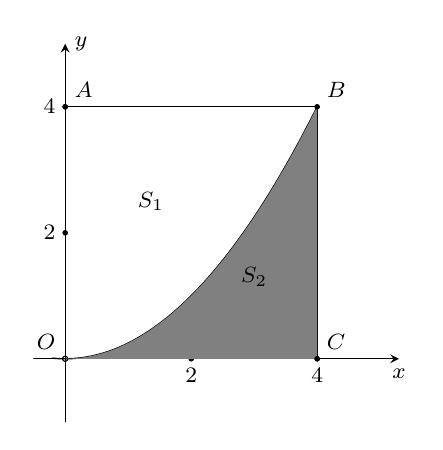
\begin{tikzpicture}[font=\footnotesize, line join=round, line cap=round, >=stealth, scale = 0.8]
		\draw[->] (-.5,0) --(0,0) node[above left]{$O$}--(5.3,0) node[below]{$x$};
		\draw[->] (0,-1) --(0,5) node[right]{$y$};
		\foreach \x in {2,4} \draw[fill] (\x,0) circle (1pt) node [below] { $\x$};
		\foreach \y in {2,4} \draw[fill] (0,\y) circle (1pt) node [left] { $\y$};
		\draw (0,0) circle (1.2pt);
		\draw[line width = 0.5pt] plot[domain=4:-.2, samples=100] (\x, {0.25*(\x)^2});
		\draw (4,0)--(4,4)--(0,4);
		\fill[gray] (0,0)-- plot[domain=0:4](\x,{0.25*(\x)^2})--(4,0)--cycle;
		\draw[fill=black] (0,4) node[above right]{$ A $} circle (1pt) (4,4) node[above right]{$ B $} circle (1pt) (4,0)node[above right]{$ C $} circle (1pt);
		\draw (1,2.5) node[right]{$ S_1 $} (3,1) node[above]{$ S_2 $};
	\end{tikzpicture}
\end{center}
\shortans{$ 2 $}
\loigiai{Ta có diện tích hình vuông $O A B C$ là $ 16 $ và bằng $S_1+S_2$.\\
Ta có $S_2=\displaystyle\int\limits_{0}^{4} \dfrac{1}{4} x^2 \mathrm{\,d} x =\left.\dfrac{x^3}{12}\right|_{0} ^{4}=\dfrac{16}{3} \Rightarrow \dfrac{S_1}{S_2}=\dfrac{16-S_2}{S_2}=\dfrac{16-\dfrac{16}{3}}{\dfrac{16}{3}}=2$.}
\end{ex}


%câu 40
\begin{ex}%[2D4V3-1]
	Cho hình thang cong $(H)$ giới hạn bởi các đường $y=\mathrm{e}^{x}$, $y=0$, $x=0$, $x=\ln 4$. Đường thẳng $x=k$, $(0<k<\ln 4)$ chia $(H)$ thành hai phần có diện tích là $S_1$ và $S_2$ như hình vẽ bên. Tìm $k$ để $S_1=2 S_2$ (làm tròn kết quả đến hàng phần chục).
	\begin{center}
		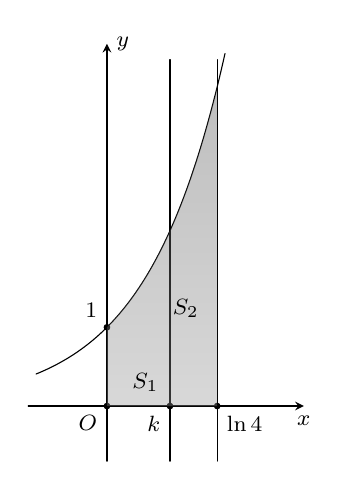
\begin{tikzpicture}[font=\footnotesize, line join=round, line cap=round, >=stealth, scale =1]
			\draw[->] (-1,0) --(0,0) node[below left]{$O$}--(2.5,0) node[below]{$x$};
			\draw[->] (0,-.7) --(0,4.6) node[right]{$y$};
			\draw[fill = black] (.8,0) node[below left]{$k$} circle (1pt);
			\draw[fill = black] (1.4,0) node[below right]{$\ln 4$} circle (1pt);
			\draw[fill = black] (0,1) node[above left]{$1$} circle (1pt);
			\draw[fill = black] (0,0) circle (1pt);
			\draw (.8,-.7)--(.8,4.4) (1.4,-.7)--(1.4,4.4);
			\draw [samples=100, domain=-.9:1.5] plot (\x, {e^(\x)});
			\fill[color=gray!10!black,shading=axis,opacity=0.2] (0,0) -- plot[smooth,samples=100,domain=0:1.4] (\x, {e^(\x)}) -- (1.4,0) -- cycle;
			\draw (0.2,.3) node[right]{$ S_1 $} (1,1) node[above]{$ S_2 $};
		\end{tikzpicture}
	\end{center}
	\shortans{$1,1$}
\loigiai{
Diện tích hình thang cong $(H)$ giới hạn bởi các đường $y=\mathrm{e}^{x}$, $y=0$, $x=0$, $x=\ln 4$ là
$$S=\displaystyle\int\limits_{0}^{\ln 4} \mathrm{e}^{x} \mathrm{\,d} x = \mathrm{e}^{x}\Bigg|_{0}^{\ln 4}=\mathrm{e}^{\ln 4}-\mathrm{e}^{0}=4-1=3.$$\\
Ta có $S=S_1+S_2=S_1+\dfrac{1}{2} S_1=\dfrac{3}{2} S_1$. Suy ra $S_1=\dfrac{2 S}{3}=\dfrac{2 \cdot 3}{3}=2$.\\
Vì $S_1$ là phần diện tích được giới hạn bởi các đường $y=\mathrm{e}^{x}$, $y=0$, $x=0$, $x=k$ nên\\
$
2=S_1=\displaystyle\int\limits_{0}^{k} \mathrm{e}^{x} \mathrm{\,d} x=\mathrm{e}^{x}\Bigg|_{0}^{k}=\mathrm{e}^{k}-\mathrm{e}^{0}=\mathrm{e}^{k}-1$.\\
Do đó $\mathrm{e}^{k}=3 \Leftrightarrow k=\ln 3 \approx 1{,}1$.}
\end{ex}

%câu 41
\begin{ex}%[2D4V3-1]
Cho hình phẳng $(H)$ giới hạn bởi các đường $y=\left|x^{2}-1\right|$ và $y=k$, với $0<k<1$. Tìm $k$ để diện tích hình phẳng $(H)$ gấp hai lần diện tích hình phẳng được kẻ sọc ở hình vẽ bên (làm tròn kết quả đến hàng phần trăm).
\begin{center}
	\begin{tikzpicture}[font=\footnotesize, line join=round, line cap=round, >=stealth, scale =1]
		\draw[->] (-2,0) --(0,0) node[below left]{$O$}--(2,0) node[below]{$x$};
		\draw[->] (0,-3) --(0,3.3) node[right]{$y$};
		\draw[fill = black] (1,0) node[below left]{$1$} circle (1pt);
		\draw[fill = black] (0,1) node[above left]{$1$} circle (1pt);
		\draw[fill = black] (0,0) circle (1pt);
		\draw (-2,.4)--(2,.4) node[above right]{$ y=k $};
		\draw [samples=100, domain=-1:1] plot (\x, {-(\x)^2+1});
		\draw [samples=100, domain=-1:-1.8] plot (\x, {(\x)^2-1});
		\draw [samples=100, domain=1:1.8] plot (\x, {(\x)^2-1});
		\draw[dashed,samples=100,domain=-1:-1.8] plot (\x, {-(\x)^2+1});
		\draw[dashed,samples=100,domain=1:1.8] plot (\x, {-(\x)^2+1});
		\fill[pattern=north west lines] (-.77,.4) -- plot[smooth,samples=100,domain=-.77:.77] (\x, {-(\x)^2+1}) -- (.77,.4) -- cycle;
		
	\end{tikzpicture}
\end{center}
\shortans{$ 0{,}59 $}
\loigiai{\begin{center}
		\begin{tikzpicture}[font=\footnotesize, line join=round, line cap=round, >=stealth, scale =1]
			\draw[->] (-2,0) --(0,0) node[below left]{$O$}--(2,0) node[below]{$x$};
			\draw[->] (0,-3) --(0,3.3) node[right]{$y$};
			\draw[fill = black] (1,0) node[below left]{$1$} circle (1pt);
			\draw[fill = black] (0,1) node[above left]{$1$} circle (1pt);
			\draw[fill = black] (0,0) circle (1pt);
			\draw (-2,.4)--(2,.4) node[above right]{$ y=k $};
			\draw [samples=100, domain=-1:1] plot (\x, {-(\x)^2+1});
			\draw [samples=100, domain=-1:-1.8] plot (\x, {(\x)^2-1});
			\draw [samples=100, domain=1:1.8] plot (\x, {(\x)^2-1});
			\draw[dashed,samples=100,domain=-1:-1.8] plot (\x, {-(\x)^2+1});
			\draw[dashed,samples=100,domain=1:1.8] plot (\x, {-(\x)^2+1});
			\fill[pattern=dots] (0,.4) -- plot[smooth,samples=100,domain=0:.77] (\x, {-(\x)^2+1}) -- (.77,.4) -- cycle;
			\fill[pattern=north west lines] (.77,.4)--plot[smooth,samples=100,domain=.77:1] (\x, {-(\x)^2+1}) -- plot[smooth,samples=100,domain=1:1.18] (\x, {(\x)^2-1}) -- (1.18,.4) -- cycle;
			\draw (0.77,.4) node[above]{$ A $} circle (1pt) (1.18,.4) node[above right]{$ B $} circle (1pt);
		\end{tikzpicture}
\end{center}
Gọi $S$ là diện tích hình phẳng $(H)$. Lúc dó $S=2 S_1+2 S_2$, trong đó $S_1$ là diện tích phần chấm bi và $S_2$ là diện tích phần gạch sọc trong hình vẽ bên.\\
Gọi $A$, $ B$ là các giao điếm có hoành độ dương của đường thẳng $y=k$ và đồ thị hàm số $y=\left|x^{2}-1\right|$, trong đó $A(\sqrt{1-k}; k)$ và $B(\sqrt{1+k}; k)$.\\
Theo yêu cầu bài toán
\begin{eqnarray*}
	& & S=2 \cdot 2 S_1 \\
	& \Leftrightarrow & S_1=S_2 \\
	& \Leftrightarrow &\displaystyle\int\limits_{0}^{\sqrt{1-k}} \left(1-x^{2}-k\right) \mathrm{\,d} x =\displaystyle\int\limits_{\sqrt{1-k}}^{1}\left(k-1+x^{2}\right) \mathrm{\,d} x+\displaystyle\int\limits_{1}^{\sqrt{1+k}}\left(k-x^{2}+1\right) \mathrm{\,d} x \\
	& \Leftrightarrow & (1-k) \sqrt{1-k}-\dfrac{1}{3}(1-k) \sqrt{1-k}=\dfrac{1}{3}-(1-k)-\dfrac{1}{3}(1-k) \sqrt{1-k}+(1-k) \sqrt{1-k}+(1+k) \sqrt{1+k}-\dfrac{1}{3}(1+k) \sqrt{1+k}-(1+k)+\dfrac{1}{3} \\
	& \Leftrightarrow &\dfrac{2}{3}(1+k) \sqrt{1+k}=\dfrac{4}{3} \\
	& \Leftrightarrow & (\sqrt{1+k})^{3}=2\\
	& \Leftrightarrow & k=\sqrt[3]{4}-1\approx 0{,}59.
\end{eqnarray*}}

\end{ex}

\Closesolutionfile{ans}
\indapan{6}{ans/ans-C4B3CD1_20-26-KQ}